\documentclass[a4paper,11pt]{article}
\usepackage[a4paper, margin=8em]{geometry}

% usa i pacchetti per la scrittura in italiano
\usepackage[french,italian]{babel}
\usepackage[T1]{fontenc}
\usepackage[utf8]{inputenc}
\frenchspacing 

% usa i pacchetti per la formattazione matematica
\usepackage{amsmath, amssymb, amsthm, amsfonts}

% usa altri pacchetti
\usepackage{gensymb}
\usepackage{hyperref}
\usepackage{standalone}

\usepackage{colortbl}

\usepackage{xstring}
\usepackage{karnaugh-map}

% imposta il titolo
\title{Appunti Sistemi Operativi}
\author{Luca Seggiani}
\date{2025}

% imposta lo stile
% usa helvetica
\usepackage[scaled]{helvet}
% usa palatino
\usepackage{palatino}
% usa un font monospazio guardabile
\usepackage{lmodern}

\renewcommand{\rmdefault}{ppl}
\renewcommand{\sfdefault}{phv}
\renewcommand{\ttdefault}{lmtt}

% circuiti
\usepackage{circuitikz}
\usetikzlibrary{babel}

% testo cerchiato
\newcommand*\circled[1]{\tikz[baseline=(char.base)]{
            \node[shape=circle,draw,inner sep=2pt] (char) {#1};}}

% disponi il titolo
\makeatletter
\renewcommand{\maketitle} {
	\begin{center} 
		\begin{minipage}[t]{.8\textwidth}
			\textsf{\huge\bfseries \@title} 
		\end{minipage}%
		\begin{minipage}[t]{.2\textwidth}
			\raggedleft \vspace{-1.65em}
			\textsf{\small \@author} \vfill
			\textsf{\small \@date}
		\end{minipage}
		\par
	\end{center}

	\thispagestyle{empty}
	\pagestyle{fancy}
}
\makeatother

% disponi teoremi
\usepackage{tcolorbox}
\newtcolorbox[auto counter, number within=section]{theorem}[2][]{%
	colback=blue!10, 
	colframe=blue!40!black, 
	sharp corners=northwest,
	fonttitle=\sffamily\bfseries, 
	title=Teorema~\thetcbcounter: #2, 
	#1
}

% disponi definizioni
\newtcolorbox[auto counter, number within=section]{definition}[2][]{%
	colback=red!10,
	colframe=red!40!black,
	sharp corners=northwest,
	fonttitle=\sffamily\bfseries,
	title=Definizione~\thetcbcounter: #2,
	#1
}

% disponi codice
\usepackage{listings}
\usepackage[table]{xcolor}

\definecolor{codegreen}{rgb}{0,0.6,0}
\definecolor{codegray}{rgb}{0.5,0.5,0.5}
\definecolor{codepurple}{rgb}{0.58,0,0.82}
\definecolor{backcolour}{rgb}{0.95,0.95,0.92}

\lstdefinestyle{codestyle}{
		backgroundcolor=\color{black!5}, 
		commentstyle=\color{codegreen},
		keywordstyle=\bfseries\color{magenta},
		numberstyle=\sffamily\tiny\color{black!60},
		stringstyle=\color{green!50!black},
		basicstyle=\ttfamily\footnotesize,
		breakatwhitespace=false,         
		breaklines=true,                 
		captionpos=b,                    
		keepspaces=true,                 
		numbers=left,                    
		numbersep=5pt,                  
		showspaces=false,                
		showstringspaces=false,
		showtabs=false,                  
		tabsize=2
}

\lstdefinestyle{shellstyle}{
		backgroundcolor=\color{black!5}, 
		basicstyle=\ttfamily\footnotesize\color{black}, 
		commentstyle=\color{black}, 
		keywordstyle=\color{black},
		numberstyle=\color{black!5},
		stringstyle=\color{black}, 
		showspaces=false,
		showstringspaces=false, 
		showtabs=false, 
		tabsize=2, 
		numbers=none, 
		breaklines=true
}


\lstdefinelanguage{assembler}{ 
  keywords={AAA, AAD, AAM, AAS, ADC, ADCB, ADCW, ADCL, ADD, ADDB, ADDW, ADDL, AND, ANDB, ANDW, ANDL,
        ARPL, BOUND, BSF, BSFL, BSFW, BSR, BSRL, BSRW, BSWAP, BT, BTC, BTCB, BTCW, BTCL, BTR, 
        BTRB, BTRW, BTRL, BTS, BTSB, BTSW, BTSL, CALL, CBW, CDQ, CLC, CLD, CLI, CLTS, CMC, CMP,
        CMPB, CMPW, CMPL, CMPS, CMPSB, CMPSD, CMPSW, CMPXCHG, CMPXCHGB, CMPXCHGW, CMPXCHGL,
        CMPXCHG8B, CPUID, CWDE, DAA, DAS, DEC, DECB, DECW, DECL, DIV, DIVB, DIVW, DIVL, ENTER,
        HLT, IDIV, IDIVB, IDIVW, IDIVL, IMUL, IMULB, IMULW, IMULL, IN, INB, INW, INL, INC, INCB,
        INCW, INCL, INS, INSB, INSD, INSW, INT, INT3, INTO, INVD, INVLPG, IRET, IRETD, JA, JAE,
        JB, JBE, JC, JCXZ, JE, JECXZ, JG, JGE, JL, JLE, JMP, JNA, JNAE, JNB, JNBE, JNC, JNE, JNG,
        JNGE, JNL, JNLE, JNO, JNP, JNS, JNZ, JO, JP, JPE, JPO, JS, JZ, LAHF, LAR, LCALL, LDS,
        LEA, LEAVE, LES, LFS, LGDT, LGS, LIDT, LMSW, LOCK, LODSB, LODSD, LODSW, LOOP, LOOPE,
        LOOPNE, LSL, LSS, LTR, MOV, MOVB, MOVW, MOVL, MOVSB, MOVSD, MOVSW, MOVSX, MOVSXB,
        MOVSXW, MOVSXL, MOVZX, MOVZXB, MOVZXW, MOVZXL, MUL, MULB, MULW, MULL, NEG, NEGB, NEGW,
        NEGL, NOP, NOT, NOTB, NOTW, NOTL, OR, ORB, ORW, ORL, OUT, OUTB, OUTW, OUTL, OUTSB, OUTSD,
        OUTSW, POP, POPL, POPW, POPB, POPA, POPAD, POPF, POPFD, PUSH, PUSHL, PUSHW, PUSHB, PUSHA, 
				PUSHAD, PUSHF, PUSHFD, RCL, RCLB, RCLW, MOVSL, MOVSB, MOVSW, STOSL, STOSB, STOSW, LODSB, LODSW,
				LODSL, INSB, INSW, INSL, OUTSB, OUTSL, OUTSW
        RCLL, RCR, RCRB, RCRW, RCRL, RDMSR, RDPMC, RDTSC, REP, REPE, REPNE, RET, ROL, ROLB, ROLW,
        ROLL, ROR, RORB, RORW, RORL, SAHF, SAL, SALB, SALW, SALL, SAR, SARB, SARW, SARL, SBB,
        SBBB, SBBW, SBBL, SCASB, SCASD, SCASW, SETA, SETAE, SETB, SETBE, SETC, SETE, SETG, SETGE,
        SETL, SETLE, SETNA, SETNAE, SETNB, SETNBE, SETNC, SETNE, SETNG, SETNGE, SETNL, SETNLE,
        SETNO, SETNP, SETNS, SETNZ, SETO, SETP, SETPE, SETPO, SETS, SETZ, SGDT, SHL, SHLB, SHLW,
        SHLL, SHLD, SHR, SHRB, SHRW, SHRL, SHRD, SIDT, SLDT, SMSW, STC, STD, STI, STOSB, STOSD,
        STOSW, STR, SUB, SUBB, SUBW, SUBL, TEST, TESTB, TESTW, TESTL, VERR, VERW, WAIT, WBINVD,
        XADD, XADDB, XADDW, XADDL, XCHG, XCHGB, XCHGW, XCHGL, XLAT, XLATB, XOR, XORB, XORW, XORL},
  keywordstyle=\color{blue}\bfseries,
  ndkeywordstyle=\color{darkgray}\bfseries,
  identifierstyle=\color{black},
  sensitive=false,
  comment=[l]{\#},
  morecomment=[s]{/*}{*/},
  commentstyle=\color{purple}\ttfamily,
  stringstyle=\color{red}\ttfamily,
  morestring=[b]',
  morestring=[b]"
}

\lstset{language=assembler, style=codestyle}

% disponi sezioni
\usepackage{titlesec}

\titleformat{\section}
	{\sffamily\Large\bfseries} 
	{\thesection}{1em}{} 
\titleformat{\subsection}
	{\sffamily\large\bfseries}   
	{\thesubsection}{1em}{} 
\titleformat{\subsubsection}
	{\sffamily\normalsize\bfseries} 
	{\thesubsubsection}{1em}{}

% tikz
\usepackage{tikz}

% float
\usepackage{float}

% grafici
\usepackage{pgfplots}
\pgfplotsset{width=10cm,compat=1.9}

% disponi alberi
\usepackage{forest}

\forestset{
	rectstyle/.style={
		for tree={rectangle,draw,font=\large\sffamily}
	},
	roundstyle/.style={
		for tree={circle,draw,font=\large}
	}
}

% disponi algoritmi
\usepackage{algorithm}
\usepackage{algorithmic}
\makeatletter
\renewcommand{\ALG@name}{Algoritmo}
\makeatother

% disponi numeri di pagina
\usepackage{fancyhdr}
\fancyhf{} 
\fancyfoot[L]{\sffamily{\thepage}}

\makeatletter
\fancyhead[L]{\raisebox{1ex}[0pt][0pt]{\sffamily{\@title \ \@date}}} 
\fancyhead[R]{\raisebox{1ex}[0pt][0pt]{\sffamily{\@author}}}
\makeatother

\begin{document}
% sezione (data)
\section{Lezione del 14-10-25}

% stili pagina
\thispagestyle{empty}
\pagestyle{fancy}

% testo
\subsection{Schedulazione real-time}
Veniamo quindi a come implementare la schedulazione nei sistemi in \textbf{tempo reale}.
Avevamo detto che questi erano sistemi principalmente di tipo \textit{embedded}, cioè incorporati, non general-purpose ma \textit{special-purpose} atti a governare sistemi esterni (sistemi di controllo per veicoli, macchinari industriali, ecc...).

\subsubsection{Esecuzione ciclica}
Abbiamo che la caratteristica principale di sistemi di questo tipo è il tipo di periferiche con cui interagiscono: invece di periferiche multiple e variabili (come nei sistemi general-purpose), avremo un insieme fisso di dispositivi di ingresso (detti \textit{sensori}) e di uscita (detti \textit{attuatori}).

Questo porta ad un paradigma di esecuzione fortemente periodico: si campiona il sistema esterno attraverso i sensori, compie una qualche elaborazione, e aggiornano gli attuatori per rispondere a quanto rilevato.

Ciò significa che i processi messi in esecuzione devono rispettare il periodo dell'esecuzione ciclica, e produrre il loro risultato entro date \textit{scadenze} date dal periodo corrente e il numero di altri processi in esecuzione.
Occorre allora avere un controllo preciso e granulare sul tempo che impiegano a terminare. 

\subsubsection{Deadline}
In questo caso prevederemo, dopo l'istante di richiesta $r$ di un processo, una certa deadline $d$, calcolata come:
$$
d = r + \Delta d
$$
dove $\Delta d$ è il tempo massimo di esecuzione del processo.
\begin{itemize}
	\item In un sistema \textit{soft real-time} si cerca di fare il possibile per assicurare che il processo termini prima di $d$;
	\item In un sistema \textit{hard real-time} la terminazione del processo prima di $d$ è prerogativa dell'integrità dell'intero sistema.
\end{itemize}

In particolare, riguardo al paradigma di esecuzione ciclica accennato nello scorso paragrafo, avremo che per un processo che deve eseguire ciclicamente con periodo $\Delta t$, per ogni istante di richiesta $r_i$ l'istante di richista successivo sarà calcolato come:
$$
r_{i + 1} = r_i + \Delta t
$$
In questo caso sarà fondamentale rispettare la diseguaglianza:
$$
d_i < r_{i + 1} \ \Leftrightarrow \ \Delta d_i < \Delta t
$$
data $d_i$ come deadline dopo la richiesta $r_i$.

Estendo il concetto a sistemi multiprogrammati, avremo che dati $n$ processi il periodo $T$ di aggiornamento simultaneo di ogni processo in esecuzione sarà:
$$
T = \text{MCM}\left(\Delta t_i\right)
$$
con $t_i$ i periodi di ogni processo: semplicemente si prende il minimo comune multiplo.

\par\smallskip

Ritornando all'idea dei CPU burst, se il processo si svolge in più CPU burst $C_1$, $C_2$, ecc... dovrà quindi essere che:
$$
T_e = \sum C_i < \Delta d_i
$$
cioè che almeno il tempo di esecuzione del processo sia minore del tempo massimo di esecuzione per rispettare la deadline corrente.

\subsubsection{Algoritmo RM}
Iniziamo quindi a vedere alcuni algoritmi di scheduling per sistemi realtime.
Il primo che vediamo è l'\textbf{RM} (\textit{Rate Monotonic}).
Questo consiste semplicemente ad assegnare una priorità statica \textit{monotonica crescente} ai processi in base al \textit{rate}, cioè la frequenza, del loro ciclo di esecuzione.
Questo equivale ad assegnare una proprietà inversamente proporzionale al periodo $t$ del processo:
$$
p \propto \frac{1}{t} = f
$$

Visto che la proprietà è statica, chiaramente l'algoritmo è non preemptive.

\par\smallskip

Facciamo quindi l'esempio dell'esecuzione dell'algoritmo, ipotizzando due processi $p_a$ e $p_b$:
\begin{table}[H]
	\center \rowcolors{2}{white}{black!10}
	\begin{tabular} { c || c | c }
		\bfseries Processo & \bfseries $\Delta \mathbf{t}$ periodo & \bfseries $\mathbf{\Delta T}$ esecuzione \\
		\hline
		$p_a$ & 2 & 1 \\ 
		$p_b$ & 5 & 1
	\end{tabular}
\end{table}

Da questo è fra l'altro immediato che, con $\Delta t_a = 2$ e $\Delta t_b = 5$, il periodo complessivo di sistema $T$ è:
$$
T = \text{MCM}(\Delta t_a, \Delta t_b) = \text{MCM}(2, 5) = 10
$$

Vedremo come questo periodo determina anche il periodo dell'attività dello scheduler.

\newpage

Simulando l'esecuzione si ha, colorando in rosso le deadline di $p_a$ e in blu quelle di $p_b$:
\begin{center}
	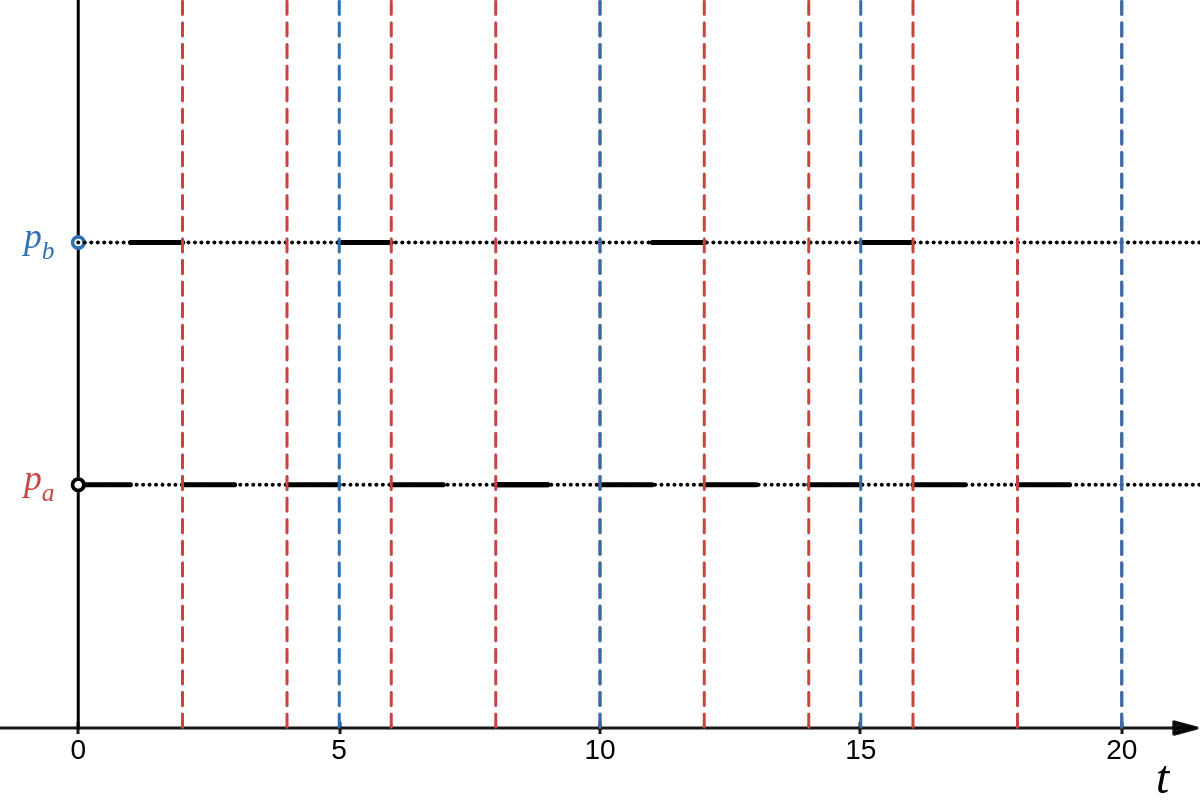
\includegraphics[scale=0.3]{../figures/rm.png}
\end{center}

Vediamo quindi come riusciamo a rispettare tutte le deadline.
Un problema è che, ad esempio all'istante 10, si sono fatti 3 cicli da un unità temporale a vuoto, cioè l'efficienza $E$ è:
$$
E = \frac{10 - 3}{10} = 70 \%
$$

Questo non è immediatamente sbagliato: significa solo che il sistema ha abbastanza risorse da soddisfare ampiamente le richieste in arrivo.
Potrebbe diventare un problema quando vogliamo \textit{"stringere"} le temporizzazioni in modo da far fronte ad un maggior numero di processi, o processi con CPU burst più consistenti.

\end{document}
